\subsection{Supervised comparator protocol and initialization controls}\label{app:pending}\label{app:slics-results}

\paragraph{Why SLiCS.}
SLiCS \citep{li2025} learns label-associated groups that reconstruct frozen
embeddings, providing a supervised decomposition control. Its v1 paper reports
no held-out MSE, VE, or original--reconstructed cosine similarity, leaving
reconstruction unquantified by those measures. Our patch adaptation uses
75 groups of three directions (225 decoder directions) and Top-16. It cannot support a capacity-matched ranking against
1,024-group models.

\paragraph{Updates and supervision.}
We adapt SLiCS Algorithm 1, which is distinct from this paper's
Algorithm~\ref{alg:agf-main}. It alternates between fitting nonnegative least
squares (NNLS) coefficients and updating individual directions by rank-one
SVD on examples where each direction contributes. We retain its conventions
for signs, clipping, and applying updates without requiring each to reduce
error. Logs record residual error and passes that increase it. Training-category
second moments provide deterministic SVD initialization. We add no separate
background group.

During fitting, SLiCS-mask permits a category's group only on patches at
least half covered by that category. SLiCS-image permits groups for all
crop-visible categories on every usable patch. We log crowd exclusions
and patches with no permitted group. Neither method needs labels at
inference. GGF instead lets all groups compete during training and uses
category information in its losses.

\paragraph{Budgets and inference.}
All arms share 2,000 training, 400 selection, 400 calibration, and 1,500
previously inspected test images, with seeds/order seeds 21--23. Ten passes
contain 500 four-image batches each. Vanilla/GGF receive 2,500 warm-up and
2,500 reconstruction/guided updates; SLiCS receives 5,000 NNLS/SVD batches.
Training-order seeds share one SVD initializer and vary data order, not
initial directions. SVD-only controls receive no alternating updates.

GGF/Vanilla use reconstruction noise scaled by 0.1; SLiCS uses clean inputs.
NNLS allows 500 iterations with tolerance $10^{-4}$. Logged projected-gradient
residuals measure distance from a stationary solution. Inference first solves
over all groups, retains the 16 strongest responses, and solves again over
those groups. Seed-21 dense inference is a separate sensitivity. Data and
decoder capacity match; total parameters, signed versus nonnegative coefficients,
floating-point operations, and runtime differ.

\paragraph{Selection and audit.}
Warm-up selects minimum MSE. Later selection maximizes capture
$+0.2\,\mathrm{AP}$ subject to MSE at most 1.02 times the common native
reference. Ineligible arms retain descriptive final-state audits. Calibration
separately chooses contrast/detector groups for frozen models, which share
test masks and patch samples. Reports retain every start/category, activity,
solver outcome, and runtime, with 200 paired image resamples. The descriptive
joint-gain rule requires positive capture gain, nonnegative AP gain, and at
most one VE point lost. This is neither an exact SLiCS retrieval reproduction nor a state-of-the-art claim.

\paragraph{Earlier initialization control.}
Run \texttt{ce65e7b00536} completes all three orders and 20 audits, including two dense sensitivities. No categories or initializations are test-selected away.

Tables~\ref{tab:small-native} and~\ref{tab:small-native-gains} compare
native-initialized GGF with continued Vanilla. Intervals use 200 valid
image draws, conditional on fixed models and reused images. Batch hashes
match. GGF adds 150 training parameters (345,975 versus 345,825).
\begin{agfresulttable}
\caption{Mean scores in the earlier 75-group comparisons. Capture, patch AP and VE are percentages. Native-initialized GGF, image-derived controls and mask-initialized models are separate experimental arms on the reused test.}\label{tab:small-native}\label{tab:image-controls}\label{tab:mask-comparison}\label{tab:mask-mean-gains}
\begin{tabular}{@{}lrrr@{}}
\toprule
Model or state & Capture (\%) & AP (\%) & VE (\%) \\
\midrule
Continued Vanilla & 9.890 & 26.068 & 51.178 \\
Native-init GGF & 15.306 & 30.647 & 51.239 \\
Image-SLiCS & 8.643 & 25.111 & 29.132 \\
Image-SVD & 16.656 & 46.506 & 35.761 \\
Mask-SLiCS & 15.876 & 50.712 & 23.775 \\
Mask-initialized GGF & 25.482 & 69.068 & 51.923 \\
Mask-SVD only & 29.528 & 79.344 & 30.211 \\
\bottomrule
\end{tabular}

\end{agfresulttable}
\begin{agfresulttable}
\caption{Native-init GGF minus continued Vanilla, percentage points. NR: interval not reported.}\label{tab:small-native-gains}\label{fig:smallcapacity-gains}
\begin{tabular}{@{}llrr@{}}
\toprule
Seed & Metric & Gain (pp) & 95\% interval \\
\midrule
21 & Capture & 5.231 & [5.073, 5.372] \\
 & Patch AP & 3.857 & [3.295, 4.622] \\
 & VE & 0.062 & \textit{NR} \\
22 & Capture & 5.185 & [5.029, 5.381] \\
 & Patch AP & 2.781 & [2.097, 3.698] \\
 & VE & 0.054 & \textit{NR} \\
23 & Capture & 5.834 & [5.643, 6.007] \\
 & Patch AP & 7.102 & [6.218, 7.982] \\
 & VE & 0.070 & \textit{NR} \\
\bottomrule
\end{tabular}

\end{agfresulttable}

Native-init GGF has lower AP than mask-SLiCS in every seed despite
better reconstruction (Table~\ref{tab:small-v-mask}). Appendix~\ref{app:maskinit}
gives the stronger mask-initialized comparison. Table~\ref{tab:image-controls}
lists image-derived controls; SVD initialization is deterministic across orders.
\begin{agfresulttable}
\caption{Native-init GGF minus mask-SLiCS: capture differences.}\label{tab:small-v-mask}
\begin{tabular}{@{}lr@{}}
\toprule
Seed & Capture change (pp) \\
\midrule
21 & $-0.246$ \\
22 & $+0.368$ \\
23 & $-1.831$ \\
\bottomrule
\end{tabular}

\end{agfresulttable}

\paragraph{Failures and interpretation.}
Both trained SLiCS arms exceed our common MSE limit at all 11 checkpoints
for every data order, so their reported final states are ineligible under
our rule. Because this limit belongs to our study rather than SLiCS, failure
does not itself imply NNLS nonconvergence. Mask-based fitting also lowers
all three mean scores relative to the SVD initializer, although the logs
do not establish the cause.

Table~\ref{tab:nnls-failures} separates training and audit
nonconvergence. Dense seed-21 inference raises VE but also activity
(Table~\ref{tab:dense-sensitivity}); it does not remove the observed trade-off.
\begin{agfresulttable}
\caption{Nonconverged NNLS calls, by order. Training uses batches; audit uses inference calls.}\label{tab:nnls-failures}
\begin{tabular}{@{}lrrrr@{}}
\toprule
Seed & Mask train & Image train & SVD audit & SLiCS audit \\
\midrule
21 & 5 & 0 & 3,050 & 0 \\
22 & 3 & 0 & 3,050 & 1 \\
23 & 8 & 0 & 3,050 & 112 \\
\bottomrule
\end{tabular}

\end{agfresulttable}
\begin{agfresulttable}
\caption{Seed-21 dense inference sensitivity, not the primary Top-16 comparison.}\label{tab:dense-sensitivity}
\begin{tabular}{@{}lrrrr@{}}
\toprule
Init. & Capture (\%) & AP (\%) & VE (\%) & Active \\
\midrule
Mask & 15.886 & 53.174 & 27.943 & 58.99 \\
Image & 8.947 & 26.180 & 37.807 & 64.77 \\
\bottomrule
\end{tabular}

\end{agfresulttable}

These finite-solver results do not establish the inferiority of published
SLiCS, even though mask-initialized GGF improves all three mean scores (Appendix~\ref{app:maskinit}).
Complete scores, validation, and solver histories remain in
\path{agf_slics_comparison_results.json}, \path{agf_slics_comparison_audit.json},
and the comparison CSVs.

\subsection{Training-mask initialization at matched capacity}\label{app:maskinit}
\begin{figure}[!htbp]
\centering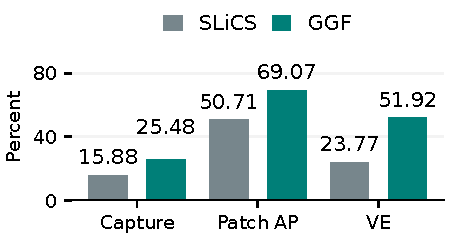
\includegraphics[width=194.4bp]{figures/agf_slics_bars.pdf}
\caption{Earlier supervised comparison with 75 three-direction groups
(225 directions): three-seed mean percentages.
Bars start at zero. The earlier SLiCS patch adaptation differs from the
published image-level method.}\label{fig:mask-slics-matched}
\end{figure}


Run \texttt{e3cf93dbe6e3} changes initialization at the comparator's 75-group,
width-three, Top-16 capacity. It retains 75 categories
and the same 2,000 training, 400 selection, 400 calibration, and 1,500
inspected-test images.

The comparator's training-mask SVD initializes the decoder, its transpose
initializes the encoder, and bias starts at zero. The second moment is
uncentered after shared normalization. Signed GGF receives 2,500 warm-up and
2,500 guided updates: Adam at 0.0003, four images, noise 0.1, and reconstruction,
contrast, and detection weights $1$, $0.05$, and $0.01$. After warm-up,
training searches all groups for fixed readouts without enforcing initial
category slots. Warm-up selects minimum MSE; guided selection maximizes
capture $+0.2\,\mathrm{AP}$ within native MSE $\times1.02$. Calibration
chooses audit groups. Every selected checkpoint meets this guard.

Seed 21 is the inspected pilot; only orders 22 and 23 are new. They share the deterministic SVD geometry and images while varying data
order and noise, with batches matched to native-initialized GGF. SLiCS uses ten alternating passes, so decoder/data matching
does not match computation or parameters.

Table~\ref{tab:mask-comparison} provides the data for Figure~\ref{fig:mask-slics-matched};
Table~\ref{tab:mask-gains} gives paired capture/AP gains. All VE differences
are positive. Intervals omit initializer-selection and training-order uncertainty.

Mean mask-initialized GGF-minus-mask-SLiCS gains are 9.607 percentage points in capture, 18.356 percentage points in patch AP and 28.148 percentage points in VE.
\begin{agfresulttable}
\caption{Mask-initialized GGF minus mask-SLiCS: paired image intervals.}\label{tab:mask-gains}
\begin{tabular}{@{}llrr@{}}
\toprule
Seed & Metric & Gain (pp) & 95\% interval \\
\midrule
21 & Capture & 9.374 & [9.049, 9.719] \\
 & Patch AP & 17.138 & [15.195, 18.452] \\
22 & Capture & 10.404 & [10.079, 10.809] \\
 & Patch AP & 19.147 & [17.227, 20.638] \\
23 & Capture & 9.042 & [8.560, 9.436] \\
 & Patch AP & 18.784 & [16.841, 20.029] \\
\bottomrule
\end{tabular}

\end{agfresulttable}

Mask-SVD alone retains higher capture and AP but lower VE
(Table~\ref{tab:mask-comparison}), so learning changes the balance rather than
improving every metric. Solver failures, MSE-limit violations, and test reuse
restrict these findings to this patch adaptation rather than published SLiCS. The final 1,024-group audit
is separate (Appendix~\ref{app:matched-baselines}). Identities, category results, and
intervals remain in \path{agf_mask_confirmation_results.json}.
